\chapter{przetwarzanie danych zebranych z odbiorników}

Przetwarzaniem danych z odbiorników zajmuje się biblioteka \textit{mp3d}
oraz program \textit{oscy} wizualizujący dane w postaci obrazu trójwymiarowego.

Biblioteka \textit{mp3d} została podzielona na pięć modułów:
\begin{enumerate}

 \item \textit{com.py} - moduł odpowiedzialny za komunikację z głównym odbiornikiem
 \item \textit{find\_pattern.py} - moduł odpowiedzialny za wyszukanie wzorca w odebranym sygnale
 \item \textit{xyz.py} - moduł odpowiedzialny za wyznaczenie pozycji i orientacji głowicy, oraz za 
 weryfikację, czy zebrane dane odpowiadają rzeczywistości
 \item \textit{info.py} - moduł wyświetlający informację o sile odbieranego sygnału
 \item \textit{ply.py} - moduł odpowiedzialny za eksportowanie danych do formaty \textit{.ply} 
    (Polygon File Format) obsługiwanego przez większość programów do obróbki grafiki 3D.

\end{enumerate}


\section{moduł \textit{com.py}}

Zadaniem modułu \textit{com.py} jest komunikacja poprzez port USB z głównym odbiornikiem,
moduł pracuje w oddzielnym wątku, w którym cyklicznie uruchamiany jest jeden z nadajników umieszczonych na głowicy,
następnie sczytuje zebrane sygnały z trzech mikrofonów umieszczonych na głównym odbiorniku.
Ta czynność powtarzana jest dla każdego z czterech nadajników. 
Zebrane dwanaście sygnałów po wstępnej filtracji przekazywane są dalej do \textit{find\_pattern.py}. Cały cykl powtarzany jest
co 200ms. Rysunek \ref{fig:com_output_2m} przedstawia sygnał przekazywany do modułu \textit{find\_pattern.py}.


\begin{figure}[h!]
    \centering
    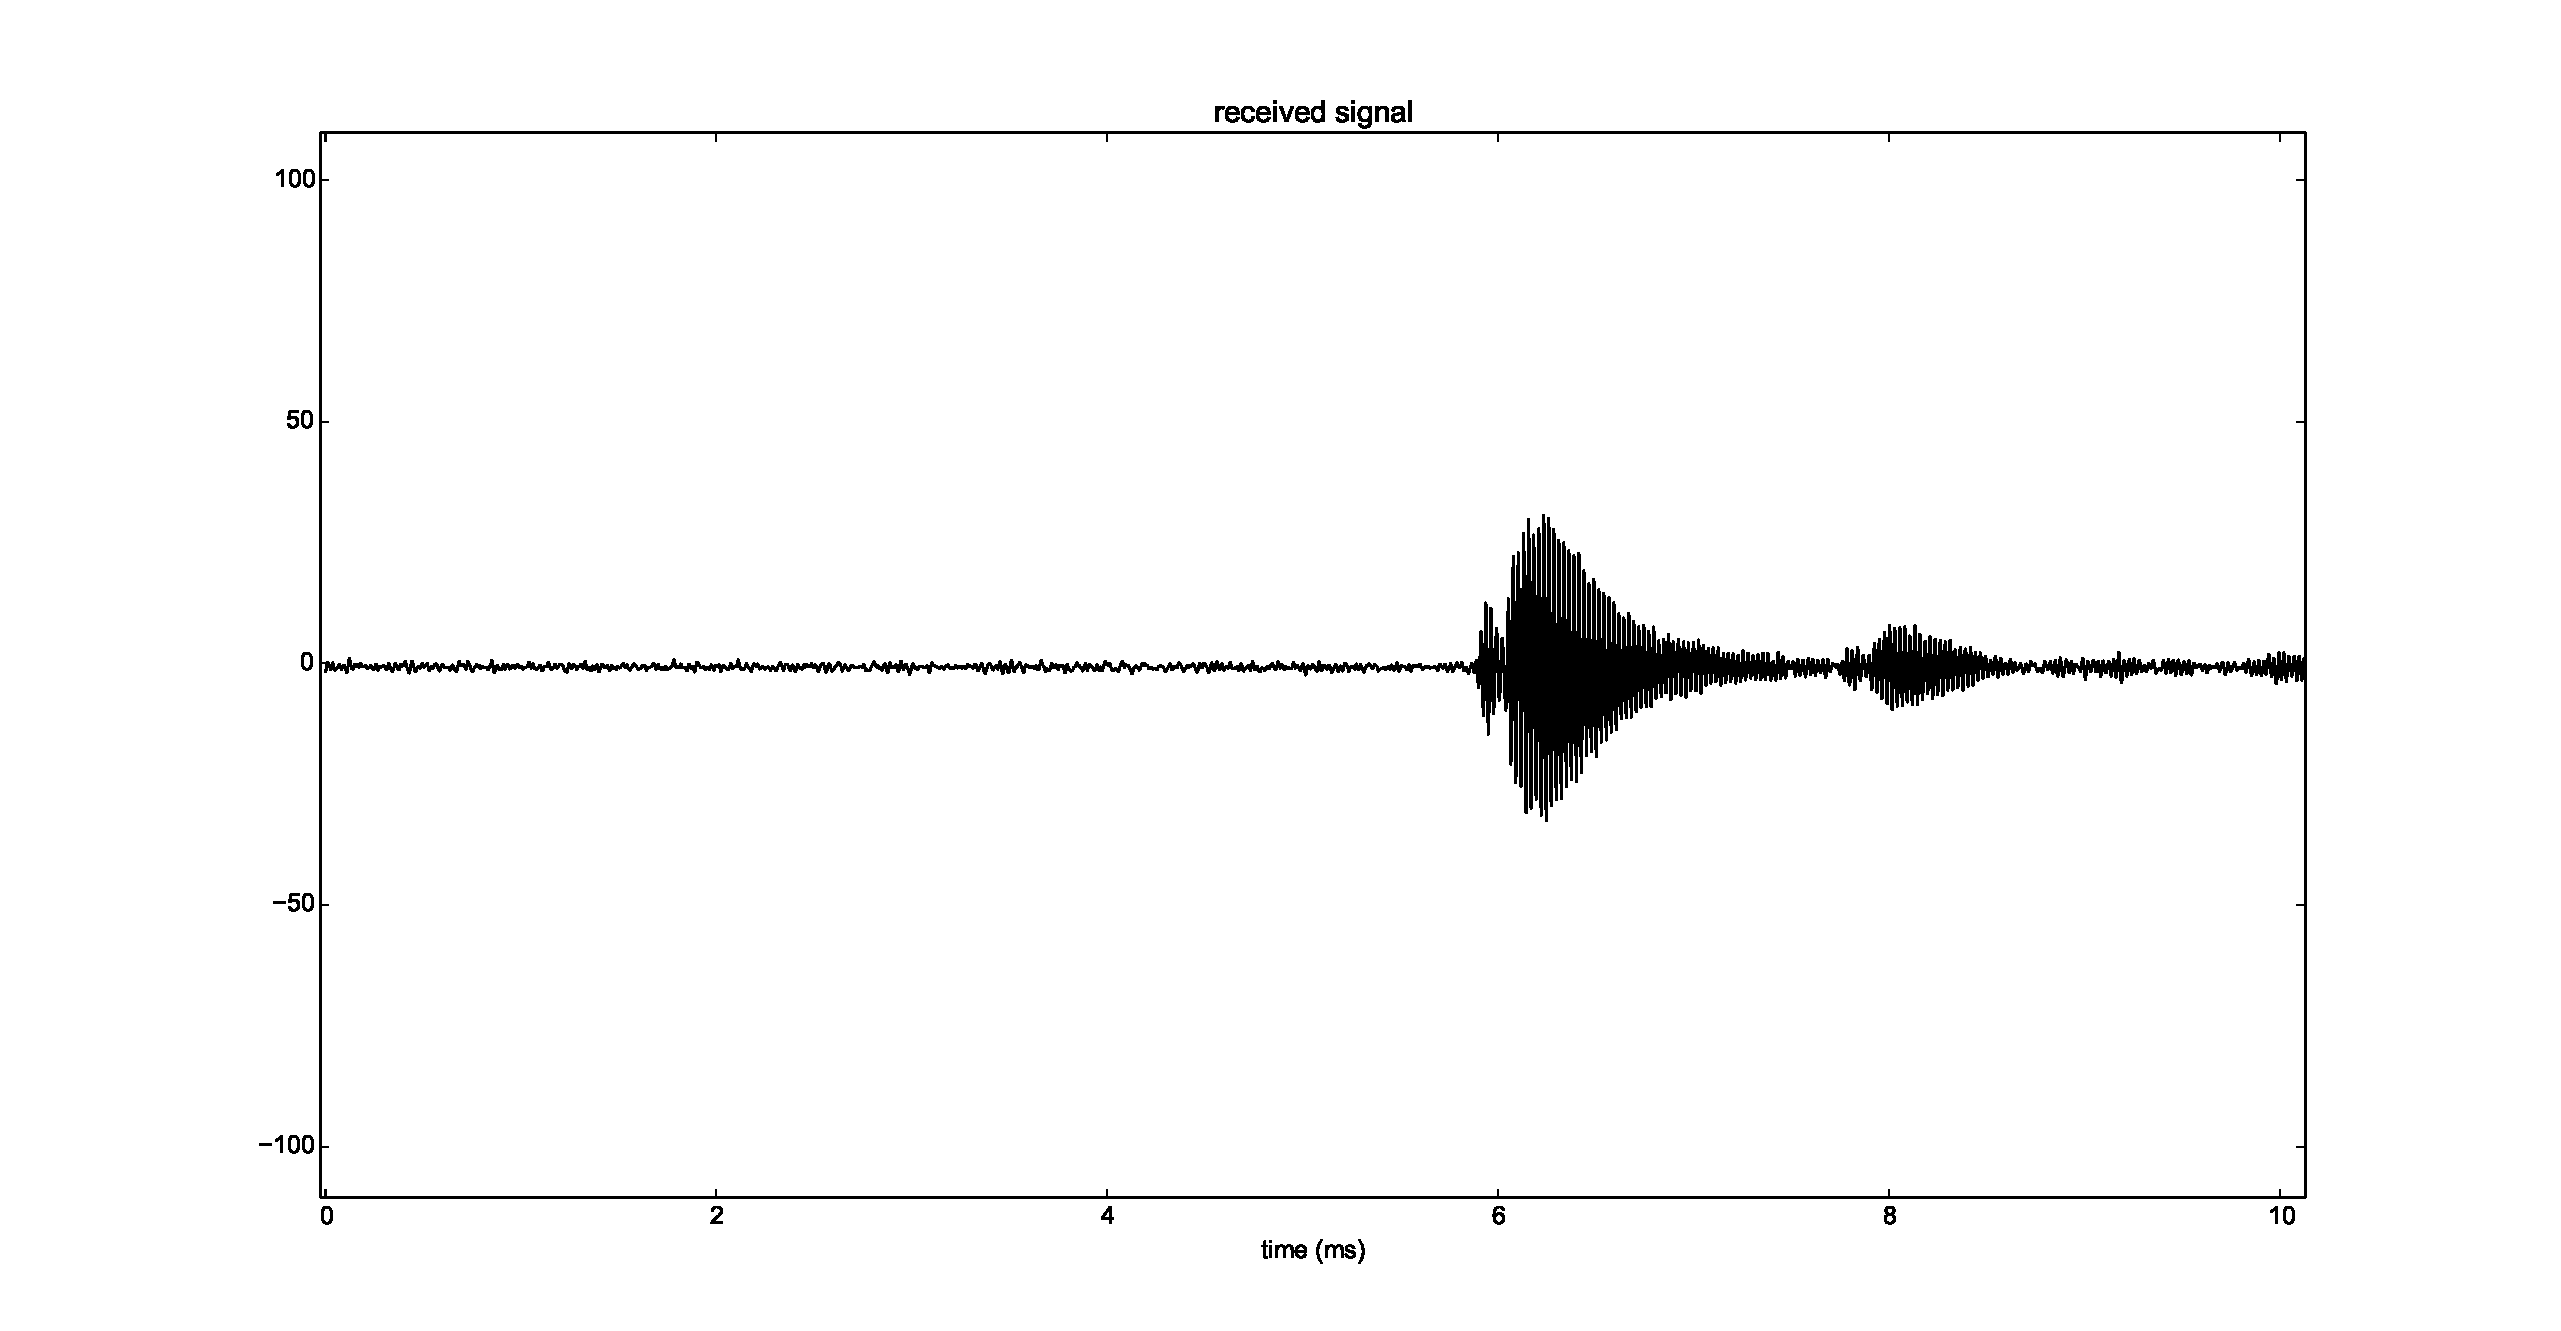
\includegraphics[width=1.15\textwidth, trim= 47mm 0mm 0mm 0mm,clip]{com_output_2m_1}
    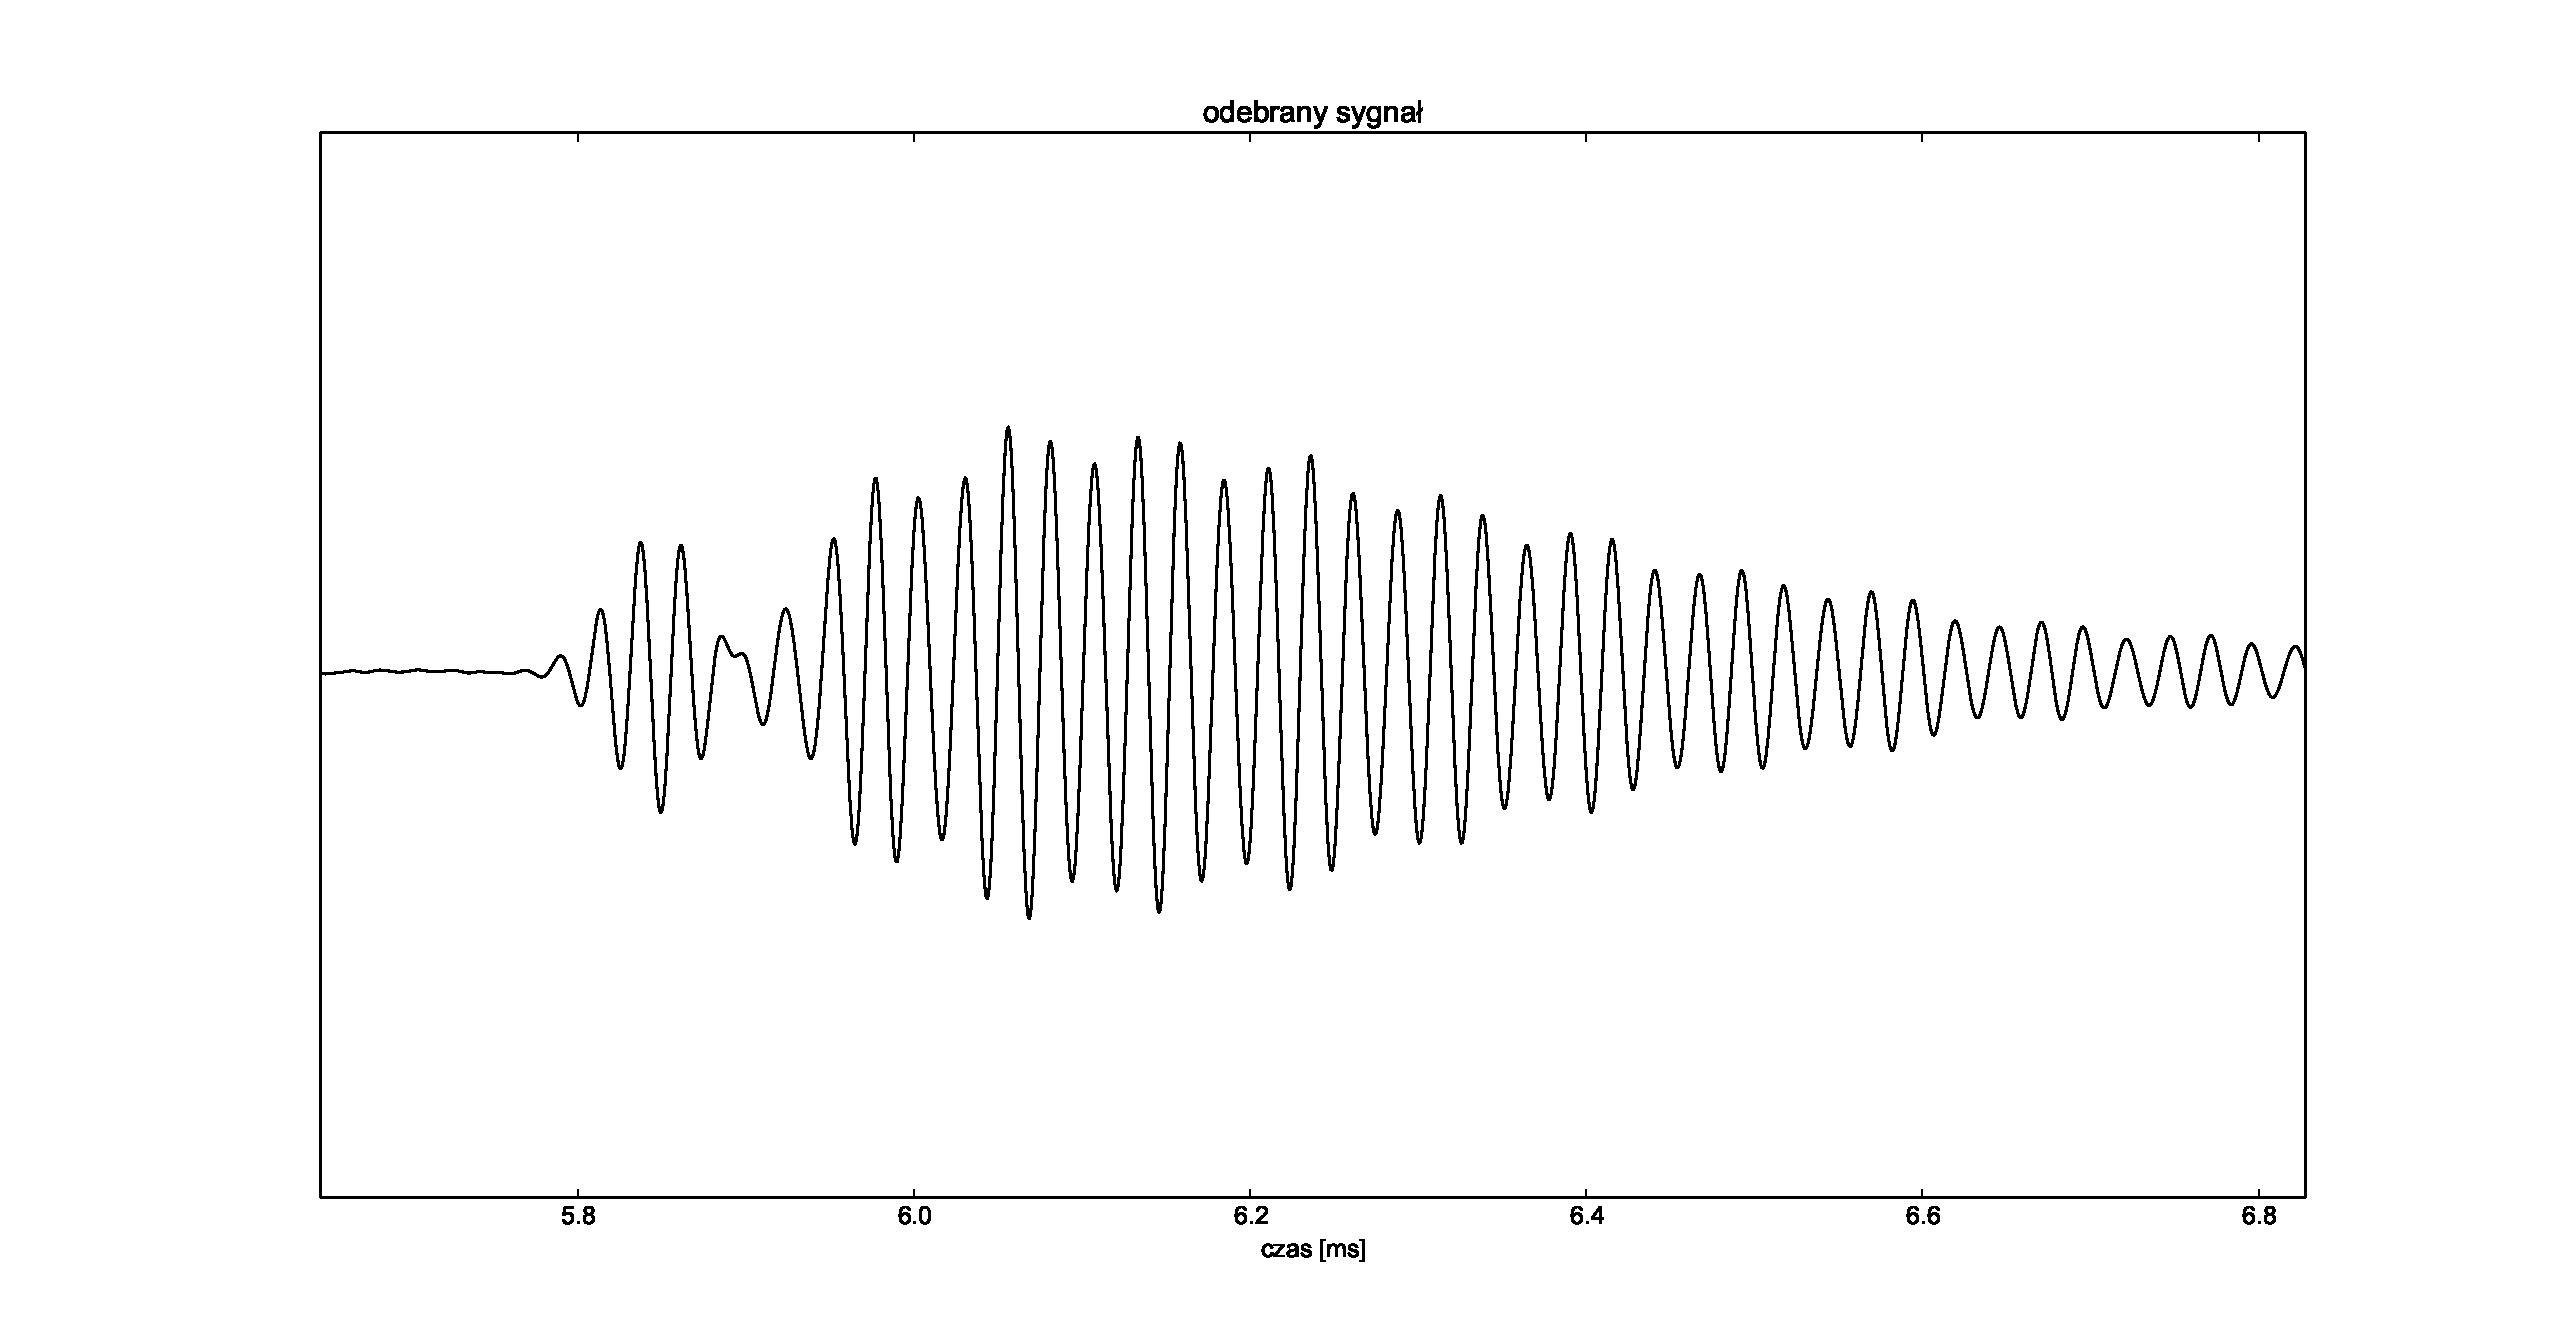
\includegraphics[width=1.15\textwidth, trim= 47mm 0mm 0mm 0mm,clip]{com_output_2m_2}
    \caption{sygnał odebrany przez moduł \textit{com.py}. 
    Odległość między nadajnikiem a odbiornikiem wynosi 2 metry.
    Na górnym wykresie po prawej stronie widoczne są również sygnały odbite od ścian.
    }
    \label{fig:com_output_2m}
\end{figure}


\section{moduł \textit{find\_pattern.py}}

Głównym modułem biblioteki \textit{mp3d} jest moduł \textit{find\_pattern.py}.
Odpowiada on za znalezienie \textit{wzorca} w odebranym sygnale z odbiorników,

Niech $w(t)$  dla $t = 0..n-1$ będzie szukanym wzorcem, a $f(x)$ odebranym sygnałem,
wtedy możemy znaleźć takie $a$, że błąd średniokwadratowy pomiędzy $w(t)$ i $a f(t+x)$ jest minimalny:
\[
  e(x) = \min_{a \in R} \{ \sum_{t=0}^{n-1}  (w(t) - a f(t+x))^2 \}
\]
zauważmy, że:
\[
  e(x) = \min_{a \in R} \{ \sum_{t=0}^{n-1}  (w^2(t) -2a w(t) f(t+x) + a^2 f^2(t+x)) \}
\]
\[
  e(x) = \min_{a \in R} \{ \sum_{t=0}^{n-1}  w^2(t) -2a \sum_{t=0}^{n-1}  w(t) f(t+x) + a^2 \sum_{t=0}^{n-1} f^2(t+x) \}
\]
funkcja kwadratowa w postaci:
\[
  y(a) = \sum_{t=0}^{n-1}  w^2(t) -2a \sum_{t=0}^{n-1}  w(t) f(t+x) + a^2 \sum_{t=0}^{n-1} f^2(t+x)
\]
osiąga minimum dla:
\[
 a = \frac{ \sum\limits_{t=0}^{n-1}  w(t) f(t+x) }{ \sum\limits_{t=0}^{n-1} f^2(t+x) }
\]
z czego ostatecznie dostajemy:

\[
  e(x) = \sum_{t=0}^{n-1}  w^2(t)  - \frac {(\sum\limits_{t=0}^{n-1}  w(t) f(t+x) )^2 } { \sum\limits_{t=0}^{n-1} f^2(t+x)}
\]

Zauważmy, że dzięki skalowaniu sygnału $f(x)$ przez parametr $a$ zamiast sygnał wzorcowy $w(x)$
otrzymany błąd $e(x)$ nie zależy od siły sygnału, co ułatwia porównanie błędów w dwóch różnych miejscach.
Ponadto wyliczenie $ \sum\limits_{t=0}^{n-1}  w^2(t) $ 
jak i $\sum\limits_{t=0}^{n-1} f^2(t+x)$ wymaga jedynie liniowej liczby operacji, a 
 $\sum\limits_{t=0}^{n-1}  w(t) f(t+x)  $ jest korelacją wzajemną funkcji $w(t)$ i $f(x)$, którą
 można wyliczyć w czasie $n \log(n)$ korzystając z szybkiej transformacji Fouriera \cite{bib:FFT_correlation}.
 
 Funkcję $e(x)$  można ją interpretować jako:
 im mniejszy błąd $e(x)$ tym większe prawdopodobieństwo, że szukany wzorzec $w$ znajduje się na pozycji $x$ w 
 odebranym sygnale $f$. 
 Wynikiem modułu \textit{find\_pattern.py} jest cała funkcja, $e(x)$ na podstawie której moduł \textit{xyz.py}
 wyznaczy pozycję głowicy w przestrzeni jak i jego orientację uwzględniając przy tym 
 kształt głowicy (nadmiarowość danych) jak i prawdopodobieństwa że znaleziony wzorzec jest na danej pozycji.
 
 Kolejną zadaniem modułu \textit{find\_pattern.py} jest uaktualnianie wzorca z biegiem czasu.
 Wraz ze zmianą kąta nachylenia nadajnika względem odbiornika zmienia się znacząco kształt sygnału,
 dlatego jeśli odnajdziemy szukany wzorzec którego moc sygnału jest wystarczająco silna to
 podmieniany jest na niego wzorzec.
 
 